\subsection{Scelte di Design} \label{sec:design-choices}
In questa sezione le scelte architetturali vengono analizzate in dettaglio, 
specificando come ci aspettiamo che il sistema verrà organizzato da un punto di vista
implementativo. Grazie a dei diagrammi UML l'applicazione prende forma negli aspetti più
tecnici che verranno poi rispettati nella fase di implementazione.

\subsubsection{Casi d'uso} \label{sec:design-choices:use-cases}
I casi d'uso espongono l'applicazione da un punto di vista strettamente funzionale,
specificando le azioni che l'utente può compiere durante le varie fasi del gioco.

In figura \ref{fig:use-cases} sono riportati i casi d'uso dell'applicazione Scala Party.
Sono suddivisi nelle schermate principali del gioco:
\begin{itemize}
    \item \textbf{Start Screen}: è la schermata iniziale del gioco, in cui l'utente
    può scegliere di iniziare una nuova partita o di visualizzare le regole del gioco.
    \item \textbf{Party Game}: è la schermata principale del gioco, in cui il giocatore
    può lanciare i dadi, muovere il proprio personaggio e ottenere gli oggetti collezionabili.
    \item \textbf{Minigame}: è la schermata in cui viene mostrato il minigioco
    attivo, in cui l'utente può visualizzare le regole e interagire con il minigioco.
\end{itemize}

\begin{figure}[ht!]
    \centering
    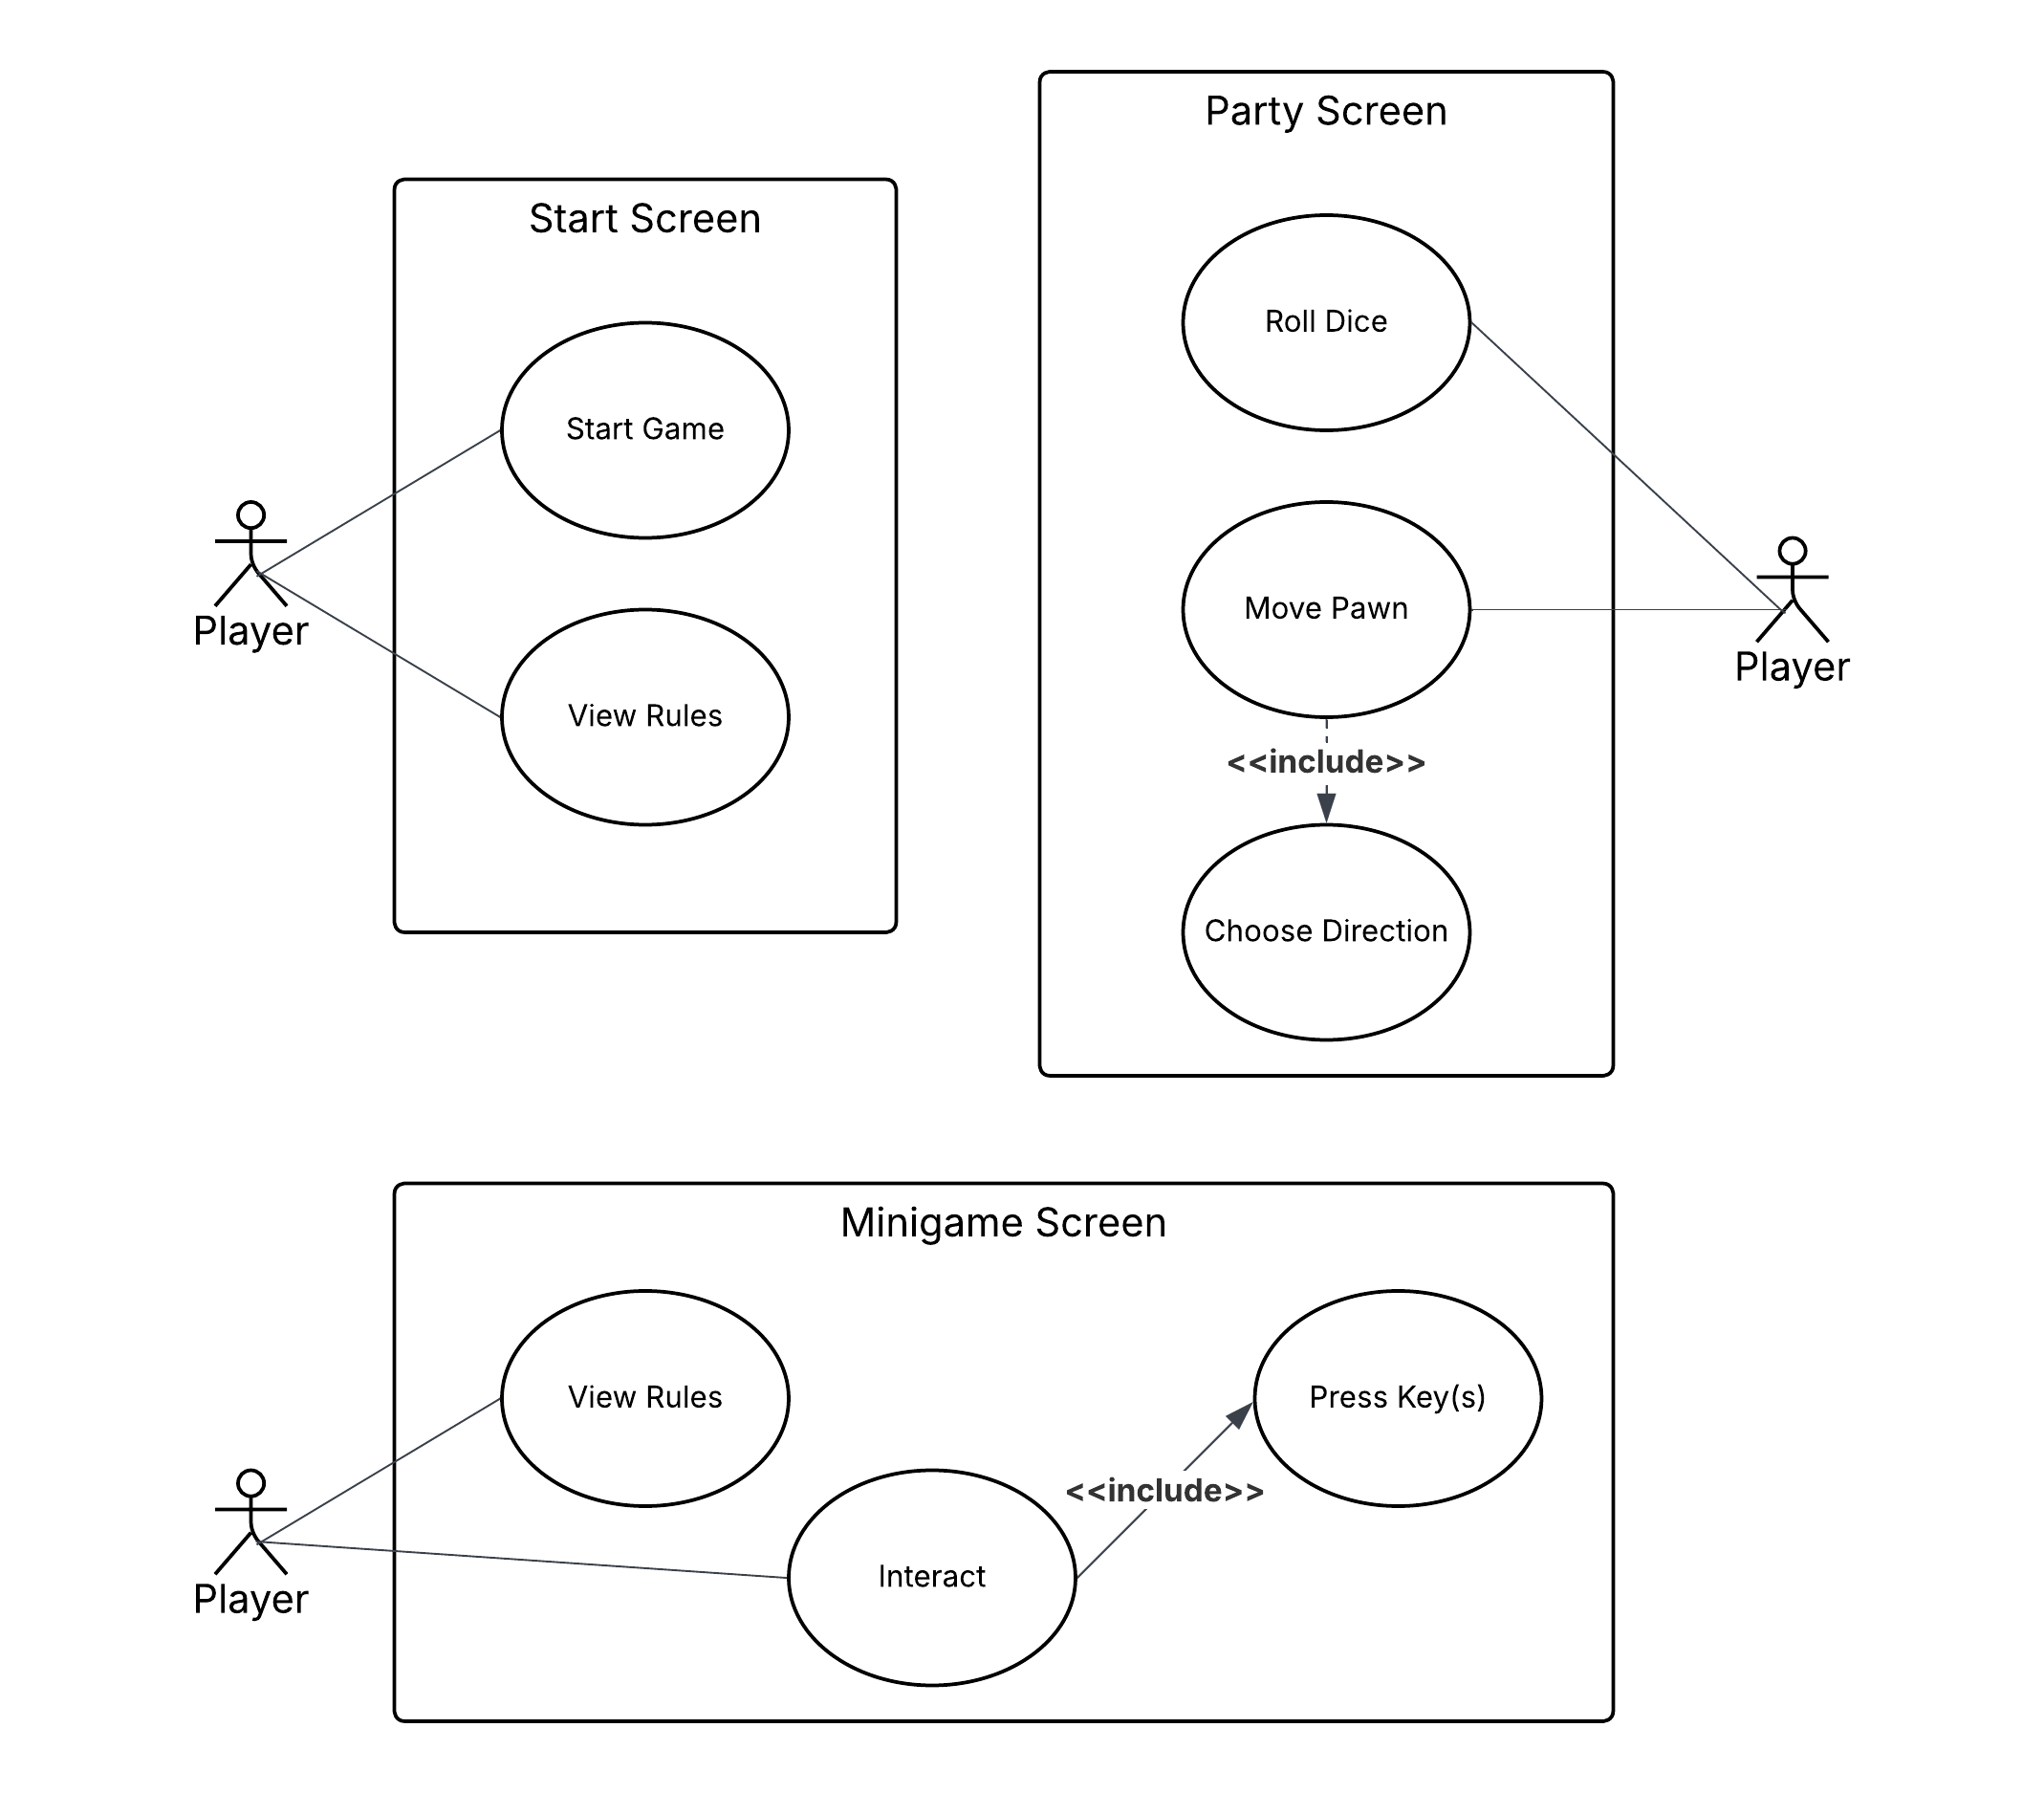
\includegraphics[width=\textwidth]{figures/use-cases.png}
    \caption{Casi d'uso dell'applicazione}
    \label{fig:use-cases}
\end{figure}

\subsubsection{Diagramma degli stati} \label{sec:design-choices:state-diagram}

\subsubsection{Diagramma delle classi} \label{sec:design-choices:class-diagram}
